% add ref biblio passive radar IEEE
\documentclass[compress,10pt]{beamer}
\usepackage{url,verbatim,amsmath}

\setbeamertemplate{background canvas}[vertical shading][bottom=white,top=structure.fg!25]
\usetheme{Hannover}
\setbeamertemplate{headline}{}
\setbeamersize{text margin left=0cm}
\graphicspath{{../../tutorials/plutosdr/2-PRN_on_PL/images/}{../gnuradioDays2019/}}

\beamertemplatefootpagenumber
\beamertemplatenavigationsymbolsempty
\definecolor{mygreen}{rgb}{0,0.6,0}

\usepackage{color}
\definecolor{grey}{rgb}{0.95,0.95,0.95}
\definecolor{keyword}{rgb}{0,0,0.95}
\definecolor{comment}{rgb}{0.95,0,0}
%\definecolor{include}{rgb}{0.55,0,0}
\definecolor{string}{rgb}{0,0.55,00.95}

\usepackage{listings}
\lstset{%backgroundcolor=\color{grey},
        language=C,
        numbers=left,
        numbersep=6pt,
        basicstyle=\tiny\ttfamily,
        extendedchars=true,
        tabsize=3,
        keywordstyle=\color{keyword}\bfseries,
        commentstyle=\color{comment},
%       includestyle=\color{include},
        stringstyle=\color{string}\itshape,
        columns=fullflexible,
        keepspaces=true
}

\setbeamertemplate{footline}{02 Feb 2020, FOSDEM 2020, Bruxelles}

\begin{document}
\date{Feb. 02, 2020}
\author[G. Goavec- Merou \& al.]{G. Goavec-Merou, J.-M. Friedt, , P.-Y. Bourgeois\\
{\footnotesize
FEMTO-ST Time \& Frequency department, Besan\c con, France \\ 
}
Contact: {\tt \{gwenhael.goavec,jmfriedt,pyb2\}@femto-st.fr} \\ \vspace{0.6cm}
\begin{center}
Slides at \\
\url{https://github.com/oscimp/oscimpDigital/tree/master/doc/conferences/fosdem2020}\\\ \\ \ \\

\includegraphics[height=1cm]{../makerspace2019/logo_femto.pdf}\vspace{-1cm}
\end{center}
}
\title[]{Platform independent CPU/FPGA co-design: the OscimpDigital framework}

\begin{frame}
\titlepage
\end{frame}

\section{Introduction}
\begin{frame}
\frametitle{Goal}

A {\bf coherent ecosystem for co-design} CPU (with Linux) and FPGA,
to assemble and generate Digital Signal Processing chains in FPGA controlled from CPU.

\begin{itemize}
\item fully pipelined chains (no FIFO): direct sample comsumption;
\item comply with GNU/Linux Operating System hierarchy (userspace application, libraries,
drivers, IP connected to the CPU);
\item vendor independent: able to handle Xilinx Vivado and Intel Quartus (may be
extended to others vendor tool)
\end{itemize}

{\bf Validated with / support:}
\begin{itemize}
\item Red Pitaya (14\&16bits): Zynq 7010 \& 7020;
\item de0nanoSoc: CycloneV Soc
\item plutoSDR: Zynq 7010
\item ADRV9361: Zynq 7035
\item USRP E310: Zynq 7020
\end{itemize}

\end{frame}
\begin{frame}
\frametitle{Existing ecosystems}
{\bf Ettus RFNoC:}\\
Pro:
\begin{itemize}
\item coherent/transparent for user (UHD abstraction);
\item enable/disable IPs at runtime (heterogeneous processing chain)
\end{itemize}
Cons:
\begin{itemize}
\item IP not available in firmware $\Rightarrow$ new bitstream to be generated;
\item limited number of blocks at the same time;
\item USRP dependent (motherboard/daughterbord/I2C EEPROM);
\item latencies introduced by crossbar
\end{itemize}

{\bf Pavel Demin red-pitaya-notes:}\\
Pro:
\begin{itemize}
\item provides plug and play projects;
\item documentation about projects;
\item direct compatibility with GNU Radio (osmosdr)
\end{itemize}
Cons
\begin{itemize}
\item dedicated to Red Pitaya platform;
\item more or less limited to provided project.
\end{itemize}

\end{frame}


%\begin{frame}\frametitle{Basics on GPS encoding}
%
%\begin{enumerate}
%\item CDMA (Code Division Multiple Access): all satellites transmit on the same frequency
%and their messages are encoded with individual orthogonal codes (Gold Codes)
%\item Satellite identification: $xcorr(signal,code)$
%\item Code orthogonality: $xcorr(code_i,code_j)=\delta_{i,j}$
%\item Doppler shift: need to compensate for remote clock frequency wrt ground clock \& local clock
%offset wrt remote atomic clocks
%\end{enumerate}
%
%\begin{center}
%\only<1>{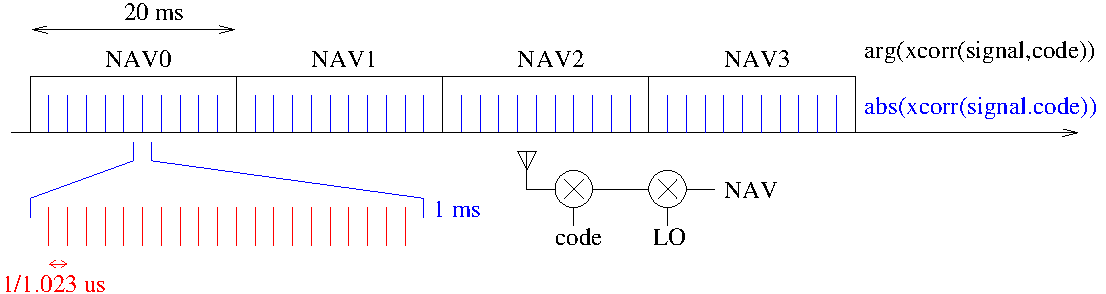
\includegraphics[width=\linewidth]{cdma}}
%\only<2>{
%\fbox{\parbox{0.8\linewidth}{
%\begin{center}
%Intensive use of correlations
%\footnote{
%Time-domain implementation on FPGA allows for pipelined computation as samples are collected
%}
% \\$xcorr(x,y)(\tau)=\int x(t)y(t+\tau)dt$ \\or through the
%convolution theorem: $FFT(xcorr(x,y)(\tau))=FFT(x)\cdot FFT(y^*)$ 
%\end{center}
%}}}
%\end{center}
%
%\end{frame}
%
%\begin{frame}[fragile]\frametitle{Basics on GPS encoding}
%
%GPS acquisition in 10~lines of Matlab program
%\footnote{\tiny using the C/A code generator
%\url{https://www.mathworks.com/matlabcentral/fileexchange/14670-gps-c-a-code-generator}} (two nested loops -- satellite number and frequency)
%
%\begin{lstlisting}[language=Matlab]
%pkg load signal
%x=read_complex_binary(filename,1024*128); fs=1.023; % sampling rate in MHz
%x=x-mean(x);
%freq0=[-10.5e3:500:10.5e3];                         % Doppler range
%time=[0:1/fs/1e6:length(x)/fs/1e6]';time=time(1:end-1);
%for m=[1:31]                                        % loop on all satellites
%   a=cacode(m,fs/1.023); a=a-mean(a);
%   l=1;
%   for freq=freq0                                   % loop on all frequency offsets
%     mysine=exp(j*2*pi*(-freq)*time); 
%     xx=x.*mysine;                                  % frequency shift the signal
%     [u(l,m),v(l,m)]=max(abs(xcorr(a,xx,'none')));  % check for cross correlation max.
%     l=l+1;
%   end
%end
%\end{lstlisting}
%
%\vspace{-0.70cm}
%\begin{minipage}[t]{\linewidth}
%\begin{minipage}{.49\linewidth}
%{\footnotesize 
%\begin{itemize}
%\item Orbital mechanics: $Doppler\in [-5000 , 5000]$~Hz
%\item Map xcorr max as a function of space vehicle number and frequency shift
%\item When a satellite is visible, sharp xcorr peak when frequency offset is compensated for
%\end{itemize}
%}
%\end{minipage}
%\begin{minipage}{.49\linewidth}
%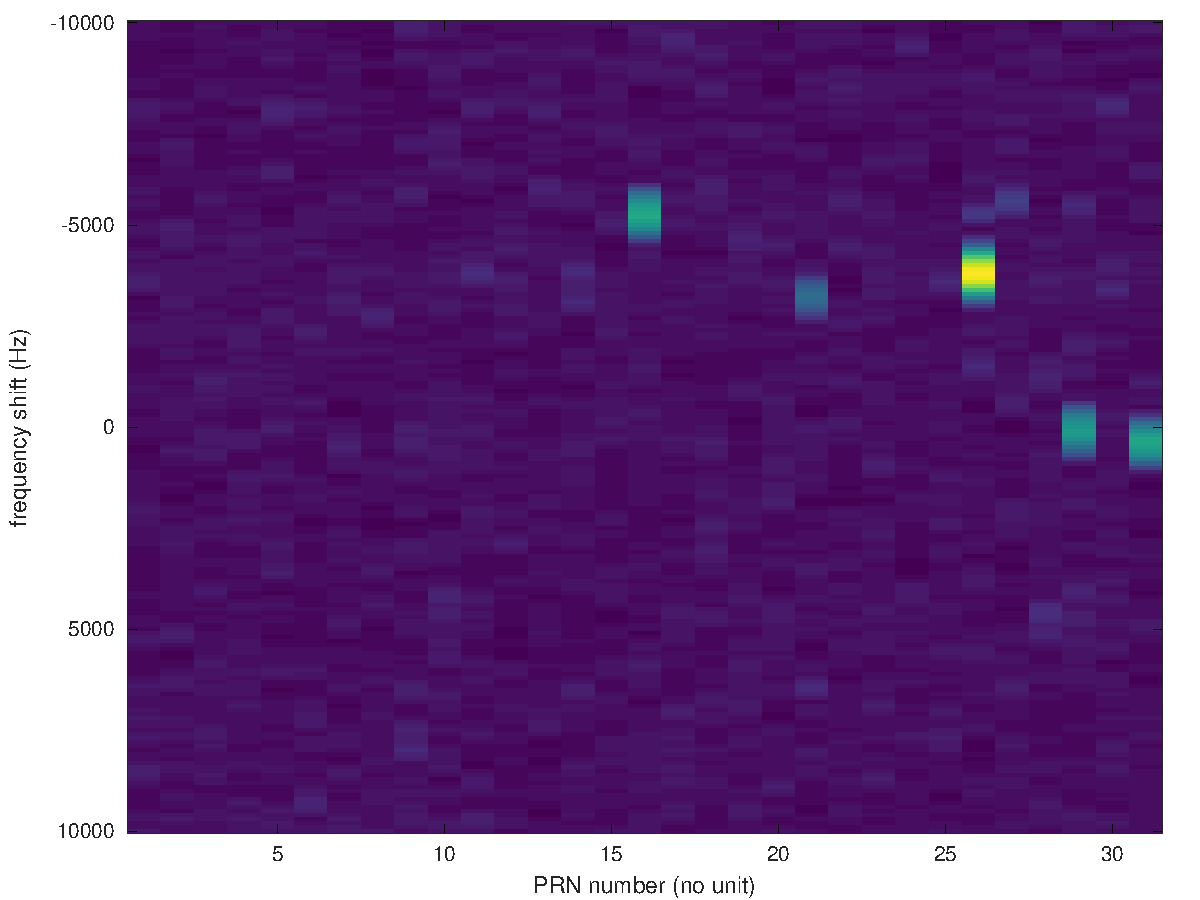
\includegraphics[width=\linewidth]{../190524gps_xcorr/gps_bin100Hz}
%\end{minipage}
%\end{minipage}
%\end{frame}
%
%\begin{frame}[fragile]\frametitle{Basics on GPS encoding}
%
%GPS acquisition in 10~lines of Matlab program (single loop on space vehicle number)
%
%\begin{lstlisting}[language=Matlab]
%pkg load signal
%x=read_complex_binary(filename,1024*128); fs=1.023; % sampling rate in MHz
%x=x-mean(x);
%freq0=[-10.5e3:500:10.5e3];                         % Doppler range
%time=[0:1/fs/1e6:length(x)/fs/1e6]';time=time(1:end-1);
%% doppler frequency shift matrix whose FFT is computed
%doppler=exp(j*2*pi*freq0'*time');                   % 43x131072 matrix
%data=ones(43,1)*x';
%all=doppler.*data;                                  % Doppler-shifted data
%allf=fft(all');
%for m=[1:31]                                        % loop on all satellites
%  a=cacode(m,fs/1.023);                             % CA code of satellite m
%  a=[a zeros(1,length(all)-length(a))];             % zero padding
%  a=a-mean(a);
%  pattern=ones(43,1)*a;                             % 43x131072 matrix
%  af=fft(pattern');
%  correlation=ifft(af.*conj(allf))';
%end
%\end{lstlisting}
%
%\vspace{-0.71cm}
%\begin{minipage}[t]{\linewidth}
%\begin{minipage}{.49\linewidth}
%{\footnotesize 
%\begin{itemize}
%\item Replace loops (inefficient) with matrix multiplication
%\item Parallelizing the frequency operations halves the computation time
%\end{itemize}
%}
%\end{minipage}
%\begin{minipage}{.49\linewidth}
%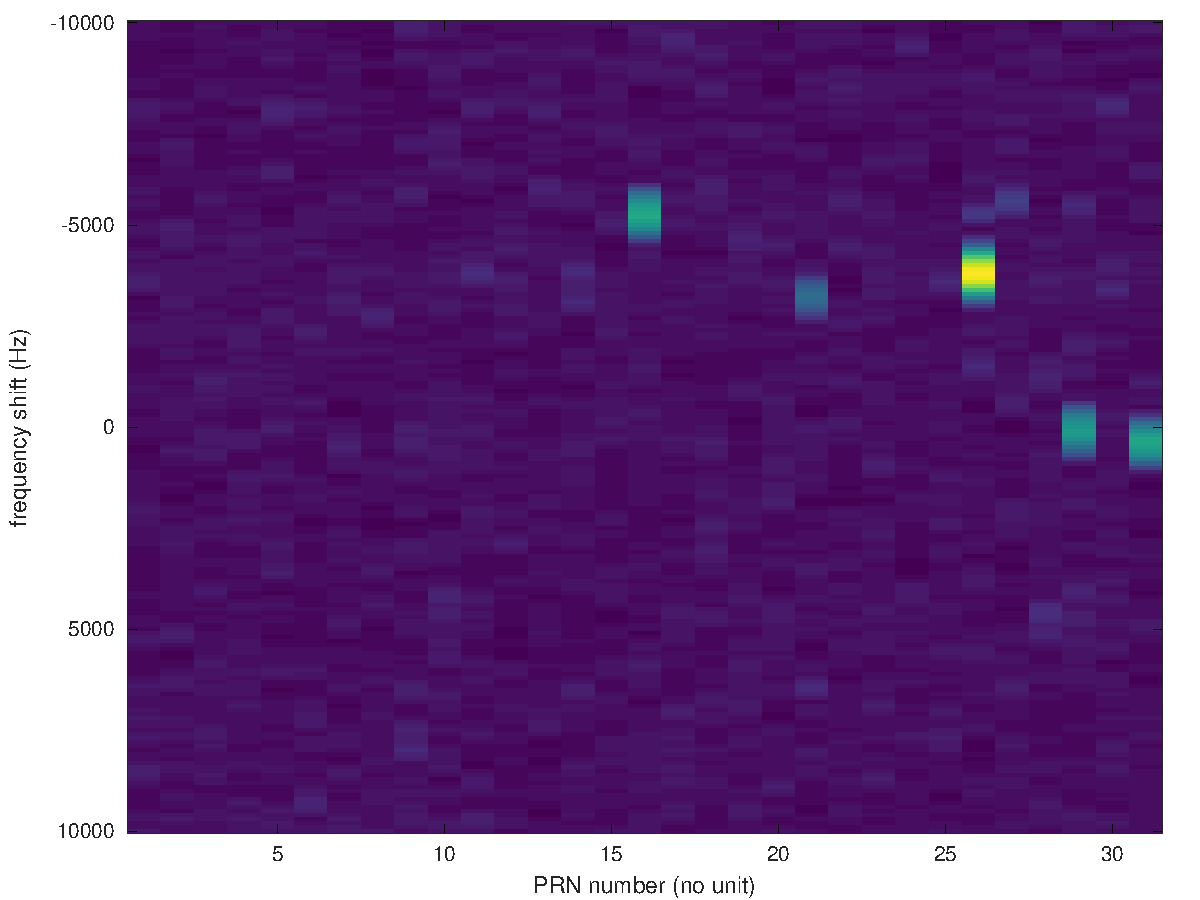
\includegraphics[width=\linewidth]{../190524gps_xcorr/gps_bin100Hz}
%\end{minipage}
%\end{minipage}
%\end{frame}
%
%\section{Embedded computation}

\section{OscimpDigital}

%\begin{frame}[fragile]\frametitle{The OscimpDigital framework}
%
%\vspace{-0.2cm}
%\hspace{-0.5cm}
%\begin{minipage}[t]{\linewidth}
%\begin{minipage}{0.8\linewidth}
%\hspace{-0.6cm}
%\begin{itemize}
%\item one algorithm $\Rightarrow$ one or more flavor (data type, performance vs.
%resources, ...): {\tt fpga\_ip} directory
%\item need to communicate between FPGA and CPU: {\tt linux\_driver} directory
%\item some IPs are widely used or complex to configure \\$\Rightarrow$ need
%to provide library with CPU code (reduce redundance, simplify application): {\tt
%liboscimp} in {\tt lib} directory.
%\end{itemize}
%\end{minipage}
%\begin{minipage}{0.1\linewidth}
%\center\includegraphics[width=2.6\textwidth]{./img/structureEco}
%\end{minipage}
%\end{minipage}
%\end{frame}

\subsection{Architecture}
\frame{\frametitle{OscimpDigital
\footnote{created thanks to the Oscillator Instability Measurement Platform (OscIMP), 
\\ \hfill \url{http://oscillator-imp.com}} ecosystem}
Purpose: provide a coherent environment to create design (FPGA), and
application (CPU):

\vspace{-0.3cm}
\begin{minipage}[t]{\linewidth}
\begin{minipage}{0.6\linewidth}
\hspace{-0.2cm}
\begin{itemize}
\item blocks (IP) with algorithm level of implementation (FPGA);
\item GNU/Linux hierarchy compliance (driver/library/application);
\item tools to generate some files and scripts/Makefile to factor most common
part.
\end{itemize}
\end{minipage}
\begin{minipage}{0.3\linewidth}
\center\includegraphics[width=0.6\textwidth]{../gnuradioDays2019/img/structureEco}
\end{minipage}
\end{minipage}
\vspace{-0.5cm}
\center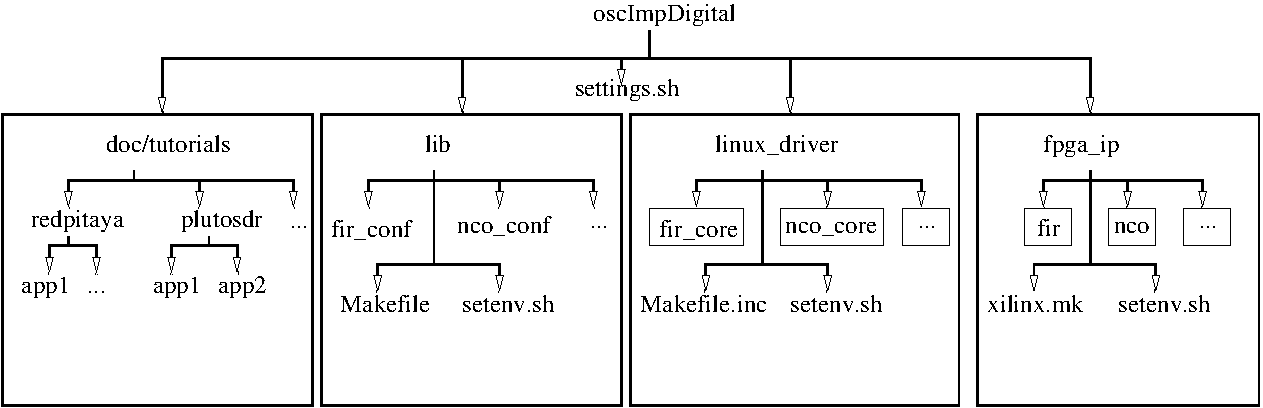
\includegraphics[width=1.0\textwidth]{../gnuradioDays2019/img/structRepo}
\vspace{-0.23cm}
}
%\frame{\frametitle{Structure}
%}
\frame{\frametitle{FPGA}
\begin{minipage}[t]{\linewidth}
\begin{minipage}{0.6\linewidth}
Algorithms or utility functions.

Developer aspect:
\begin{itemize}
\item normalize interfaces between blocks
\item isolation between implementation and communication
\end{itemize}

End user aspect:
\begin{itemize}
\item 0, 1 or more interface to connect;
\item AXI interface automatically connected.
\end{itemize}
\end{minipage}
\begin{minipage}{0.35\linewidth}
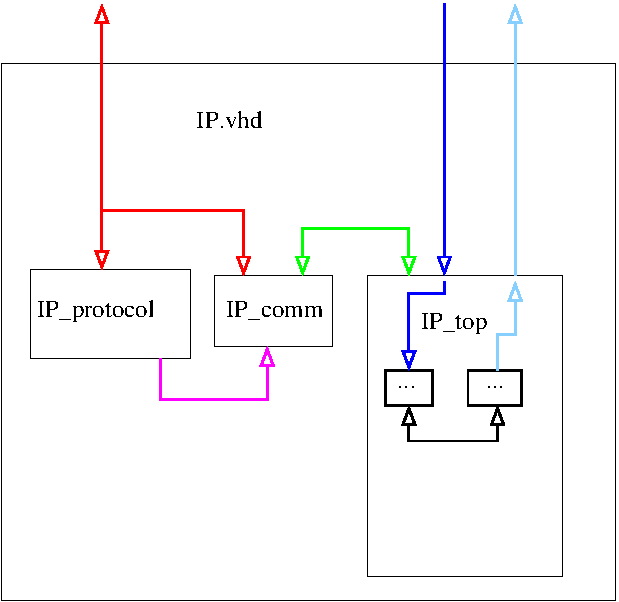
\includegraphics[width=1.2\textwidth]{../gnuradioDays2019/img/structureIp}
\end{minipage}
\end{minipage}
\begin{center}
\only<1>{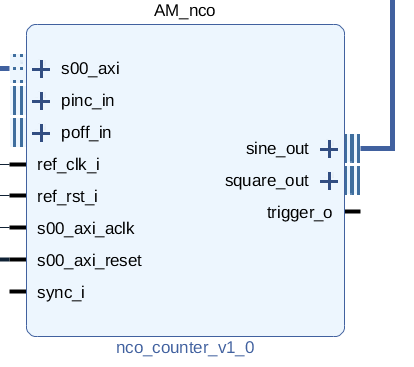
\includegraphics[width=0.4\textwidth]{./interfaceClose}}
\only<2>{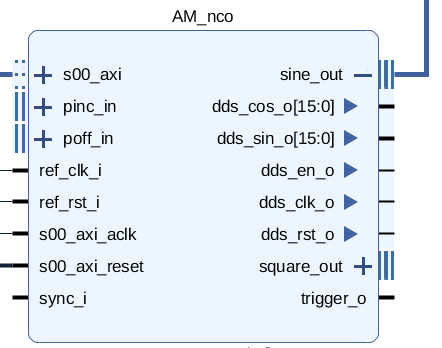
\includegraphics[width=0.4\textwidth]{./interfaceOpen}}
\only<3>{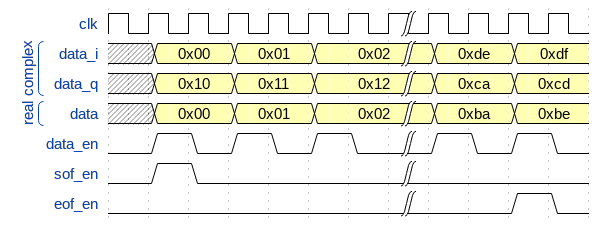
\includegraphics[width=0.9\textwidth]{../gnuradioDays2019/img/displayIf}}
\end{center}
}
%\frame{\frametitle{CPU: environment}
%{\bf Char device drivers} to add abstraction, GNU/Linux hierarchy compliance and
%communication improvement:
%\begin{itemize}
%\item 1 IP with communication $\Rightarrow$ 1 (or more) driver(s);
%\item a {\tt core} driver knows how to communicate with an IP but not where;
%\item {\tt device tree overlay} used to provide which drivers must be probed and
%base address for each of them;
%\end{itemize}
%TODO $\Rightarrow$ IIO integration
%
%{\bf libraries} to simplify some common and long (number of line) tasks.
%}

\subsection{TCL scripting}
\begin{frame}[containsverbatim]
\frametitle{Independant TCL set}
All vendor tools have a TCL mode, but:
\begin{itemize}
\item each vendor provides custom functions
\item way to build project/block design are differents
\end{itemize}

$\Rightarrow$ need to provide an set of functions and Makefile to have add an
abstraction.

\begin{minipage}[t]{\linewidth}
\begin{minipage}{0.5\linewidth}
\parbox{0.9\linewidth}{
\begin{itemize}
\item same script may be used with different boards for different manufacturers;
\item only need to reimplement a few procedures for supporting a new tool
\end{itemize}
}
\end{minipage}
\begin{minipage}{0.5\linewidth}
Vivado:
\begin{lstlisting}[language=TCL,basicstyle=\tiny]
create_bd_cell -type ip -vlnv ggm:cogen:myIP myip]
set_property -dict [ list CONFIG.PARAM1 14 \
    CONFIG.PARAM2 true ] myIP
\end{lstlisting}

Quartus:
\begin{lstlisting}[language=TCL,basicstyle=\tiny]
add_instance myip myIP 1.0
set_instance_parameter_value myip PARAM1 14
set_instance_parameter_value myip PARAM2 true
\end{lstlisting}

OscimpDigital:
\begin{lstlisting}[language=TCL,basicstyle=\tiny]
add_ip_and_conf myIP myip {
    PARAM1 14 PARAM2 true}
\end{lstlisting}

Makefile:
\begin{lstlisting}[language=make,basicstyle=\tiny]
PRJ=myGateware
CONSTR_redpitaya=leds.xdc   # use for Red Pitaya board
CONSTR_de0nanoSoc=leds.tcl # use for de0nanoSoc board
TCL_LIST=myScript.tcl
-include $(OSCIMP_DIGITAL_IP)/fpga_ip.mk

\end{lstlisting}

\end{minipage}
\end{minipage}
\end{frame}

\frame{\frametitle{Project structure}

\parbox{1.05\linewidth}{
\begin{itemize}
\item TCL script or GUI generated FPGA design
\item devicetree ({\tt .dts}) provides list of drivers and base addresses;
\item {\tt Makefile} to cross-compile application \& generate the {\tt dtbo} from dts
\item {\tt applicationName\_us.sh}: a shell script used to flash FPGA, load devicetree
and drivers;
\item {\tt main.c}: user application
\end{itemize}
}

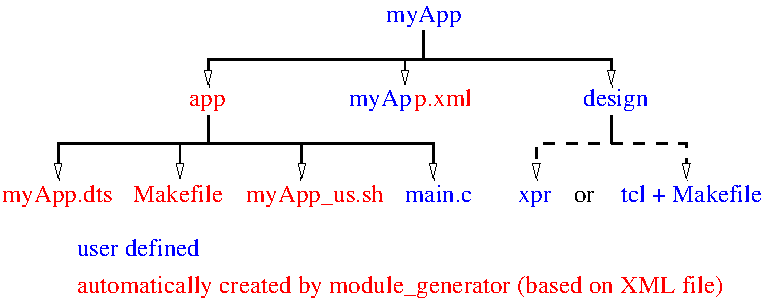
\includegraphics[width=1.0\textwidth]{../gnuradioDays2019/img/structApp.pdf}
}

%\begin{frame}[containsverbatim]
%\frametitle{CPU: module\_generator}
%\begin{itemize}
%\item Used to generate some files in {\tt app/} directory.
%\item use an XML file for design's informations.
%\end{itemize}
%
%{\small \verb!module_generator -dts myApp.xml!}
%
%\hspace{-0.6cm}
%%\begin{columns}[t]
%%\begin{column}{0.57\textwidth}
%%myApp.xml
%%\vspace{-0.2cm}
%{\footnotesize \begin{verbatim}
%<?xml version="1.0" encoding="utf-8"?>
%<project name="tutorial5" version="1.0">
%  <options>
%    <option target="makefile" name="USE_STATIC_LIB">1</option>
%    <option target="makefile" name="LDFLAGS">-liio</option>
%  </options>
%  <ips>
%    <ip name ="dataComplex_to_ram" >
%      <instance name="data1600" id = "0"
%        base_addr="0x43c00000" addr_size="0xffff" />
%    </ip>
%    <ip name ="nco_counter">
%      <instance name="nco" id = "0"
%        base_addr="0x43c10000" addr_size="0xffff" />
%    </ip>
%  </ips>
%</project>
%\end{verbatim}
%}
%\end{frame}

\begin{frame}[containsverbatim]
\frametitle{CPU: module\_generator}
\begin{itemize}
\item Used to generate some files in {\tt app/} directory.
\item use an XML file for design information.
\end{itemize}

{\footnotesize \verb!module_generator -dts myApp.xml!}

%\vspace{-0.5cm}
\hspace{-0.6cm}
\begin{columns}[t]
\begin{column}{0.50\textwidth}
myApp.xml
\vspace{-0.2cm}
{\tiny \begin{verbatim}
<?xml version="1.0" encoding="utf-8"?>
<project name="tutorial5" version="1.0">
  <ips>
    <ip name ="data_to_ram" >
      <instance name="data1600" id = "0"
        base_addr="0x43c00000" addr_size="0xffff" />
    </ip>
    <ip name ="nco_counter">
      <instance name="datanco0" id = "0"
        base_addr="0x43c10000" addr_size="0xffff" />
    </ip>
  <ips>
</project>
\end{verbatim}
}

tutorial5\_us.sh
\vspace{-0.2cm}
{\tiny
\begin{verbatim}
cp ../bitstreams/tutorial5_wrapper.bit.bin /lib/firmware
rmdir /sys/kernel/config/device-tree/overlays/fpga
mkdir /sys/kernel/config/device-tree/overlays/fpga
cat tutorial5.dtbo > $DTB_DIR/dtbo
insmod ../../modules/data_to_ram_core.ko
insmod ../../modules/nco_counter_core.ko
\end{verbatim}
}
\end{column}
\begin{column}{0.60\textwidth}
tutorial5.dts
\vspace{-0.3cm}
{\tiny
\begin{verbatim}
/dts-v1/;
/plugin/;
/ {
    compatible = "xlnx,zynq-7000";
    fragment0 {
        target = <&fpga_full>;
        #address-cells = <1>;
        #size-cells = <1>;
        __overlay__ {
            #address-cells = <1>;
            #size-cells = <1>;
            firmware-name = "tutorial5_wrapper.bit.bin";
            data1600: data1600@43c00000{
                compatible = "ggm,dataToRam";
                reg = <0x43c00000 0xffff>;
            };
            datanco0: datanco0@43c10000{
                compatible = "ggm,nco_counter";
                reg = <0x43c10000 0xffff>;
            };
        };
    };
};
\end{verbatim}
}
\vspace{-0.2cm}
Makefile
\vspace{-0.3cm}
{\tiny
\begin{verbatim}
BASE_NAME=tutorial5
CORE_MODULES_LIST=$(OSCIMP_DIGITAL_DRIVER)/nco_core/*.ko \
        $(OSCIMP_DIGITAL_DRIVER)/data_to_ram_core/*.ko
include $(OSCIMP_DIGITAL_APP)/Makefile.inc

\end{verbatim}
}
\end{column}
\end{columns}

\end{frame}

\begin{frame}\frametitle{Available processing blocks}
{\footnotesize
{\bf Radiofrequency signal handling}
\begin{itemize}
\item nco\_counter \hfill local oscillator
\item mixerComplex\_sin, mixer\_sin \hfill frequency transposition
\item redpitaya\_converters \hfill Red Pitaya platform hardware interfaces
(in/out)
\item axi\_deltaSigma \hfill low frequency output (audio output)
\item gen\_radar\_prog, syncTrigStream \hfill pulsed RADAR, synchronization
\end{itemize}

{\bf Radiofrequency signal processing}
\begin{itemize}
\item cacode \hfill GPS Gold code generator
\item firReal \hfill CPU configurable Finite Impulse Response filter
\item prn, prn20b, xcorr\_prn\_slow\_complex \hfill pseudo-random sequence
generator, correlator
\end{itemize}

{\bf Two types of interfaces: real values and complex values (*: valid
for both types):}
\begin{itemize}
\item add\_const*, adder\_substracter\_*, mean* \hfill linear operations
\item convertComplexToReal, convertRealToComplex \hfill type conversion
\item duppl*\_1\_to\_2 \hfill stream splitting
\item expander*, shifter* (bit shifts) \hfill bit shifts
\item switch* \hfill flow control
\end{itemize}

{\bf Interface between real/complex and AXI bus or CPU:}
\begin{itemize}
\item axiStreamTo*, *ToAxiStream, axi\_to\_dac \hfill AXI to complex/real
\item data*\_to\_ram, data*\_dma\_direct \hfill FPGA$\rightarrow$CPU
communication
\end{itemize}
}
% slv_to_sl_axi ?!
\end{frame}

\section{Application examples}
\subsection{GPS acquisition}
\begin{frame}\frametitle{Why SDR-based GNSS decoding~?}

\begin{enumerate}
\item Flexibility of adding new features without updating hardware
\item Beyond timing \& positioning: access to the raw I/Q stream
\begin{itemize}
\item basic physics (reflectometry)
\item security (phased array for spoofing detection)
\item 1575.42~MHz within range of the PlutoSDR (AD9363 + Zynq SoC)
\end{itemize}
\end{enumerate}

\vfill
\begin{center}
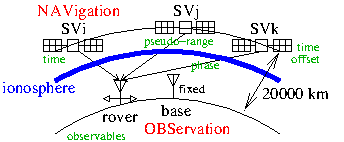
\includegraphics[width=.7\linewidth]{fig2}\\
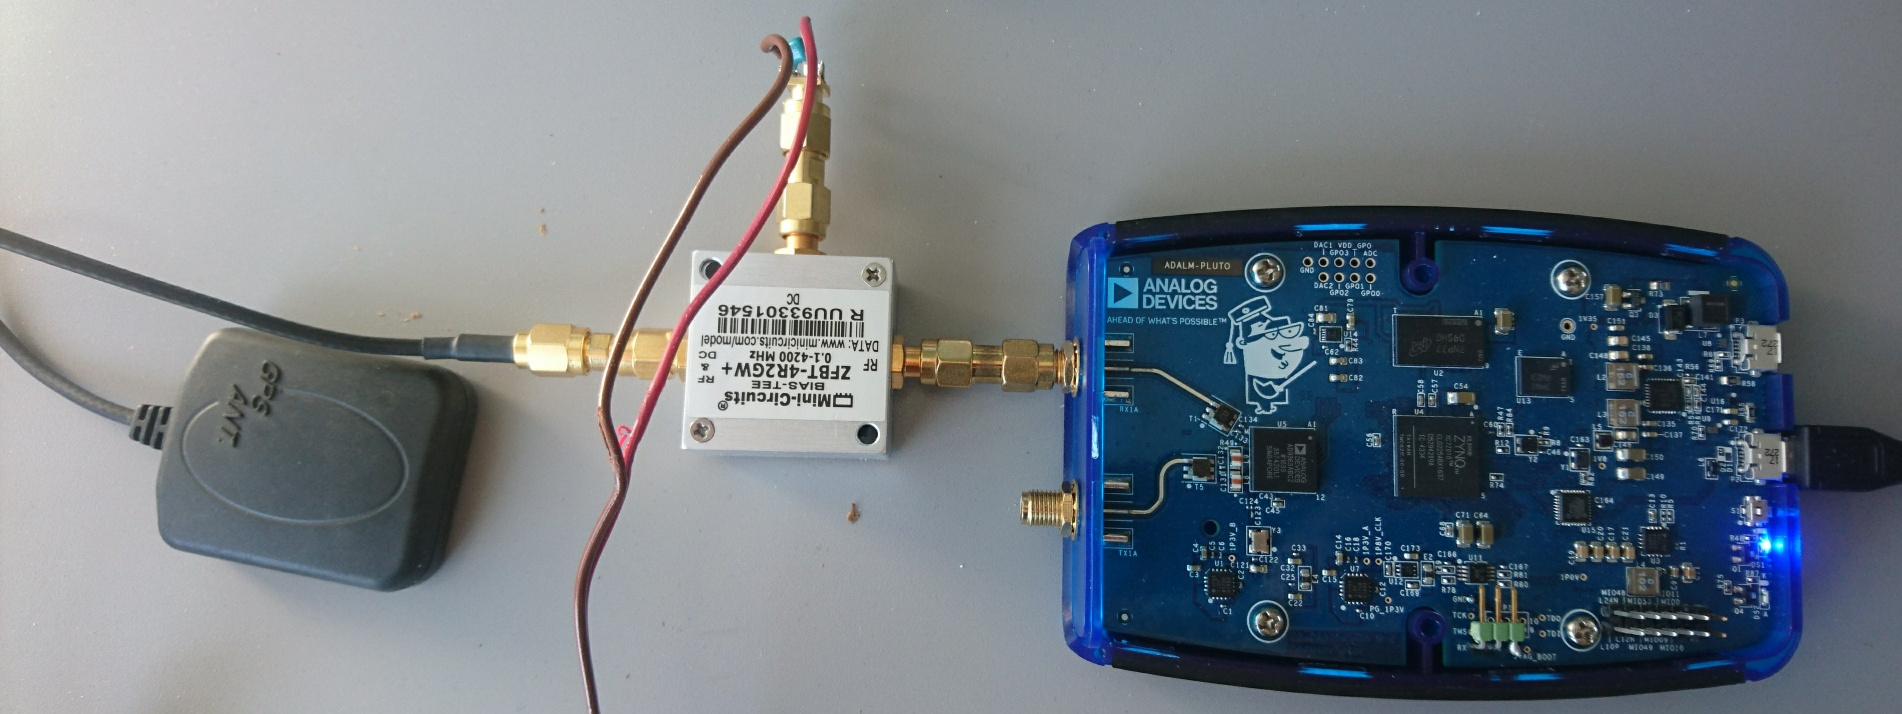
\includegraphics[width=.7\linewidth]{DSC_0279.JPG}
\end{center}

\end{frame}
\begin{frame}[fragile]\frametitle{Using the embedded FGPA}

\begin{itemize}
\item
GNU/Octave implementation: 1 to 2 second/satellite \\
$\Rightarrow$ $\simeq$1~min for acquisition depending on frequency steps
\item The PlutoSDR Zynq official firmware
is only used for data collection and transfer to the PC (bandwidth
{\bf limited by USB})
\item Preprocessing on the Zynq FPGA {\bf removes the communication bandwidth bottleneck}
\item Making best use of the available resources on the embedded FPGA (PL)
\item Possible additional pre-processing on the embedded CPU (PS) running GNU Radio before sending
over USB
\end{itemize}

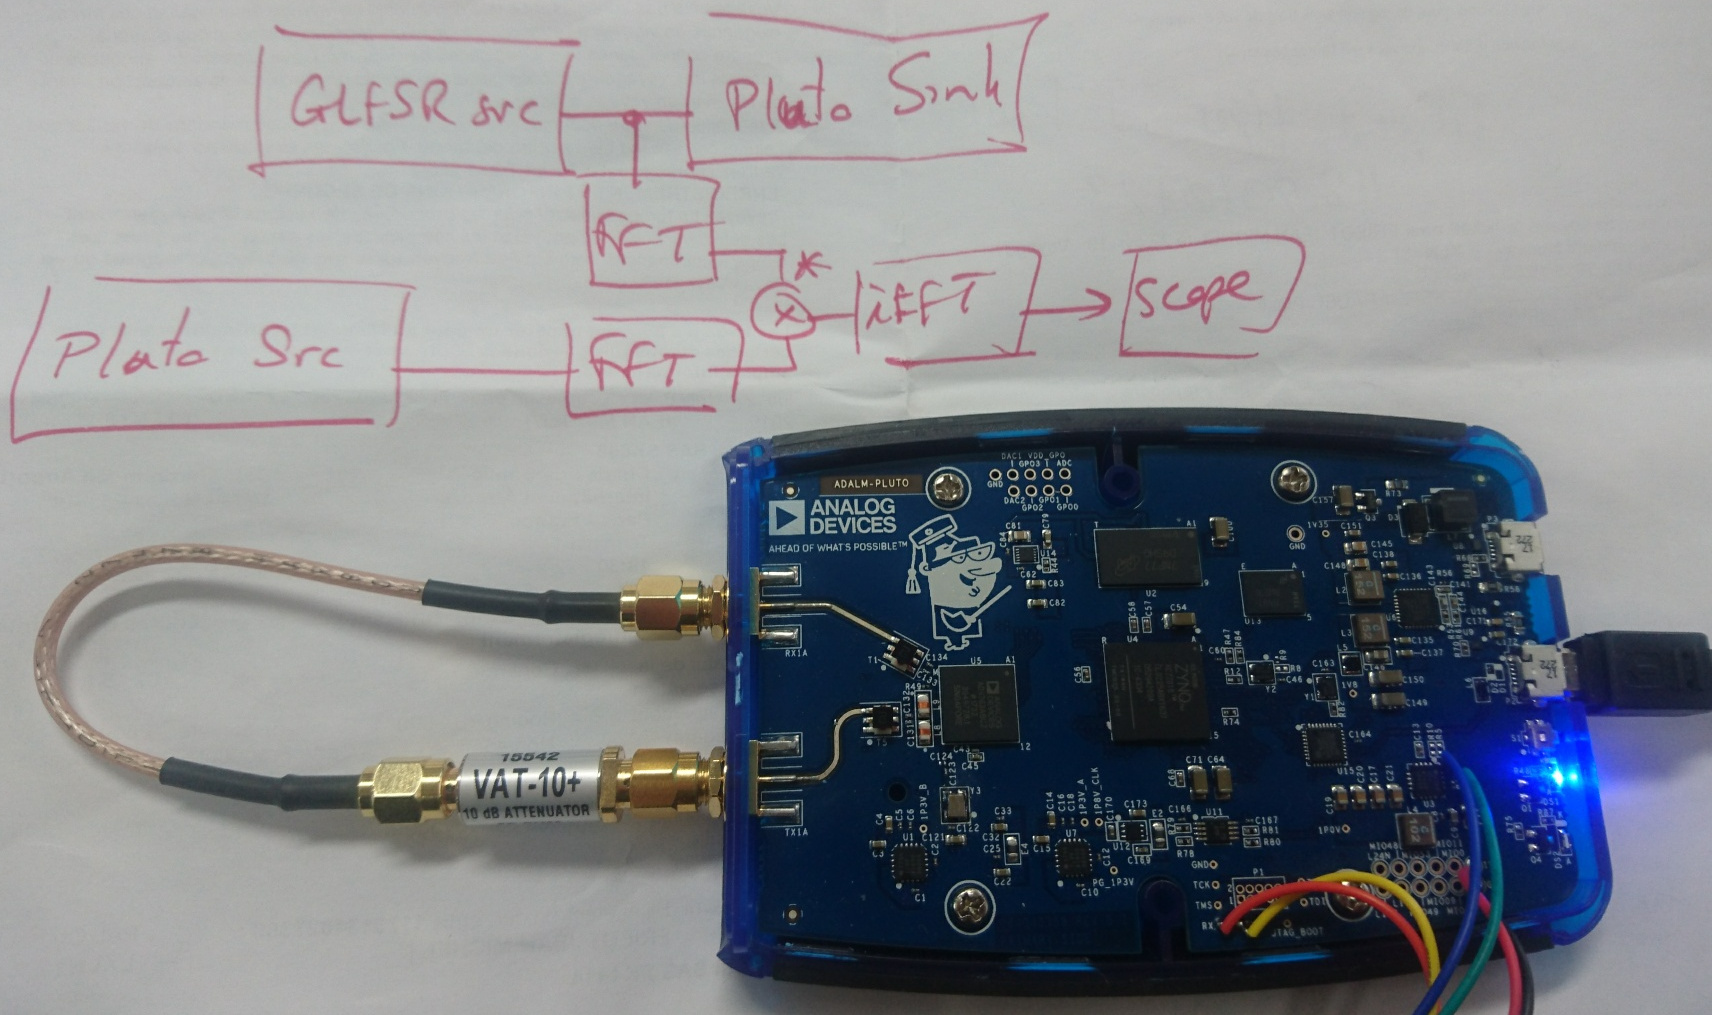
\includegraphics[width=.31\linewidth]{DSC_0275.JPG}
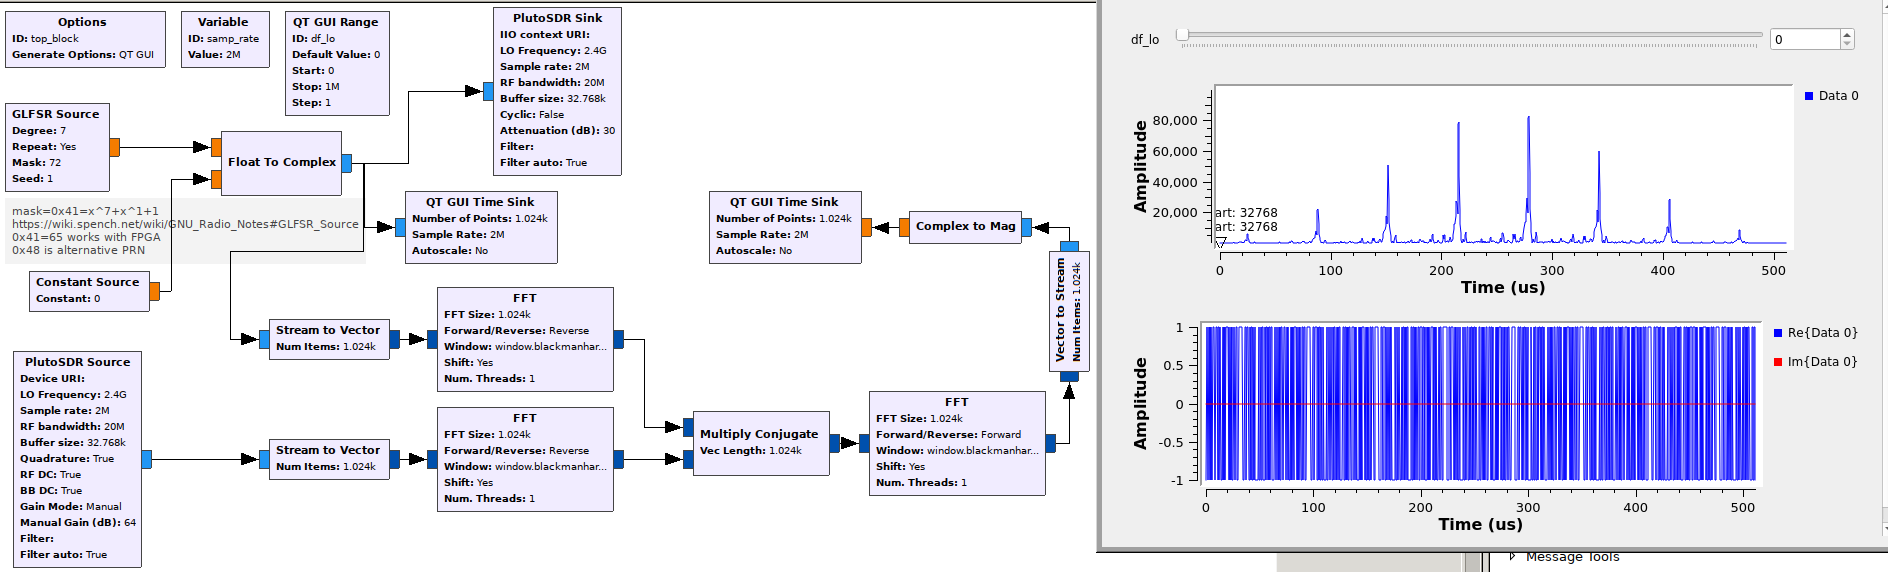
\includegraphics[width=.68\linewidth]{xcorr_pluto2}
\end{frame}

\begin{frame}[fragile]\frametitle{Principle}

\begin{center}
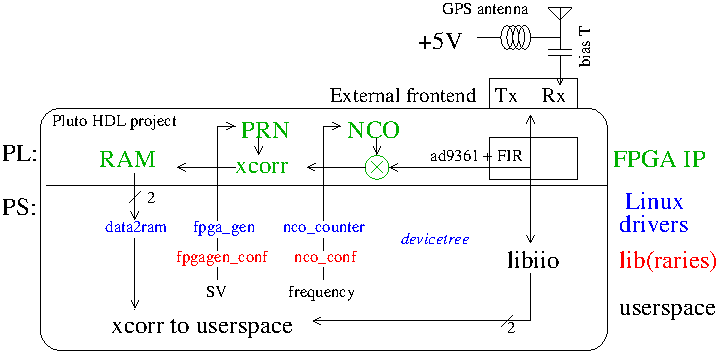
\includegraphics[width=\linewidth]{plutopluto-oscimpDigital-makerspace}
\end{center}

\begin{itemize}
\item PL: collect data from AD9363, frequency transposition (NCO), Gold Code generation \& correlation
\item PS: loop frequency, loop space vehicle number, fetch correlation, control AD9363 (libiio)
\end{itemize}

Complex interaction between FPGA processing blocks and processor userspace through
Linux drivers (modules)
\end{frame}
\begin{frame}[fragile]\frametitle{Application to GPS decoding}

\begin{itemize}
\item
TCL scripts define the processing functions, their settings and how they are 
connected to each other
\item Zynq on the PlutoSDR $\Rightarrow$ Xilinx Vivado (despite platform
independence of OscimpDigital)
\end{itemize}

\begin{center}
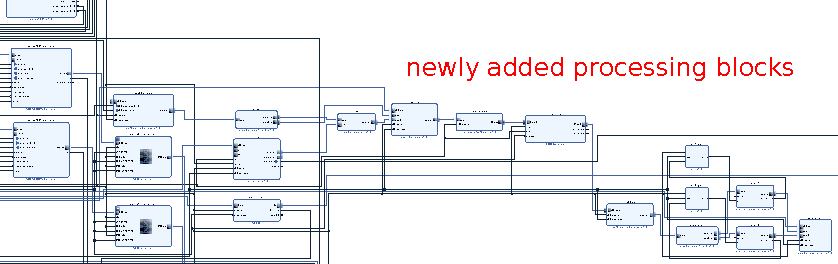
\includegraphics[width=1.0\linewidth]{2xcorr_2PRN_NCO_crop.pdf}
{\footnotesize Dual PRN generator and cross-correlation with the received datastream frequency
transposed using the NCO.\par}
\end{center}

\vfill
{\bf 22~s on Zynq PL} (limited by the FPGA area limiting the number of parallel correlations) v.s {\bf 108~s on 2.6 GHz PC} (GNU/Octave)

{\bf $\Rightarrow$ move to ADRV9361 to have more resources (WIP)}
\end{frame}

\subsection{Autonomous FM receiver}
\begin{frame}
\frametitle{PlutoSDR: embedded broadcast FM receiver with audio card output
\footnote{\url{https://github.com/oscimp/oscimpDigital/tree/master/doc/tutorials/plutosdr/99-gnuradio-audio}}}
\vspace{0.2cm}
\begin{minipage}[t]{\linewidth}
\begin{minipage}{.50\linewidth}
\begin{itemize}
\item GNU Radio in PlutoSDR firmware
\item add sound card IP in parallel to processing chain
\item Python or C++ flowgraph
\end{itemize}
\end{minipage}
\begin{minipage}{.50\linewidth}
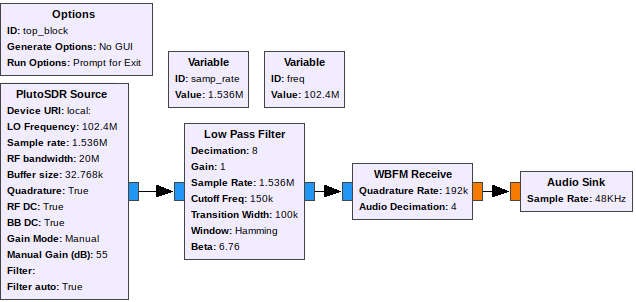
\includegraphics[width=1.0\textwidth]{pluto_embedded_audio.png}\\
\end{minipage}
\end{minipage}
\begin{center}
\vspace{-0.4cm}
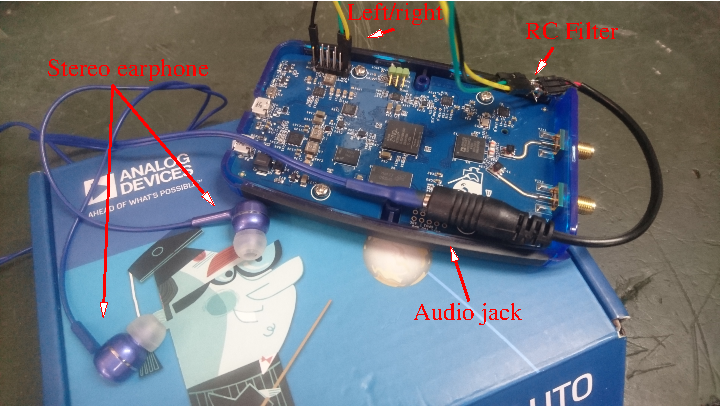
\includegraphics[width=0.55\textwidth]{../../tutorials/plutosdr/99-gnuradio-audio/figures/pluto_audio_ann.pdf}
\end{center}
\end{frame}

\begin{frame}
\frametitle{PlutoSDR: embedded broadcast FM receiver with audio card output}

\begin{minipage}[t]{\linewidth}
\begin{minipage}{.50\linewidth}
\hspace{-0.8cm}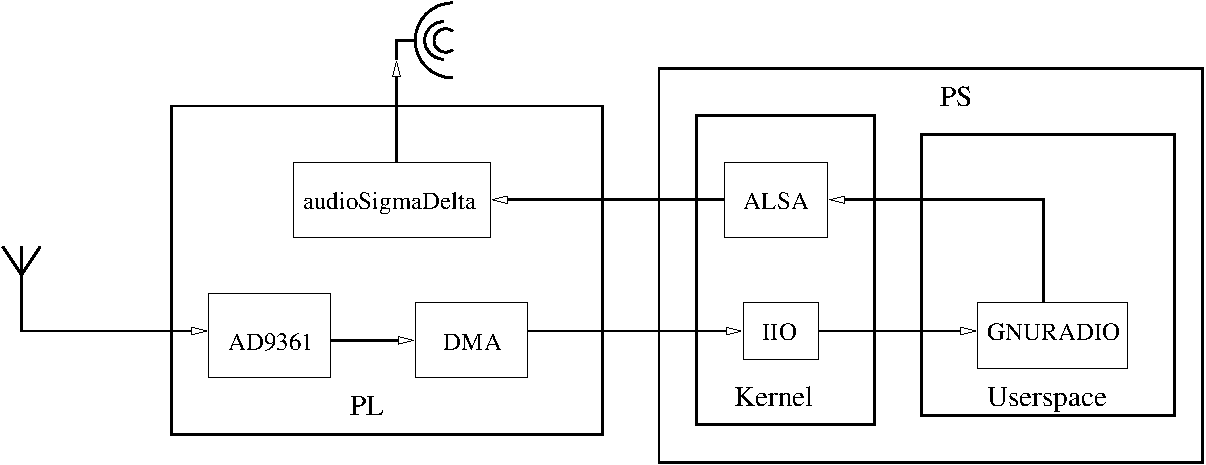
\includegraphics[width=1.2\textwidth]{plutoSchema.pdf}
\end{minipage}
\begin{minipage}{.50\linewidth}
\begin{itemize}
\item dual sigma-delta IP for stereo output
\item alsa compatible driver
\item use local iio backend
\end{itemize}
\end{minipage}
\end{minipage}

\vfill
\begin{minipage}[t]{\linewidth}
\begin{minipage}{.50\linewidth}
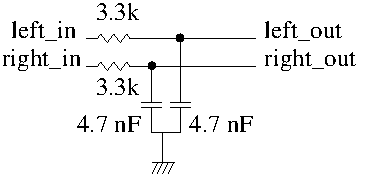
\includegraphics[width=1.\textwidth]{RC_filter.pdf}
\end{minipage}
\begin{minipage}{.50\linewidth}
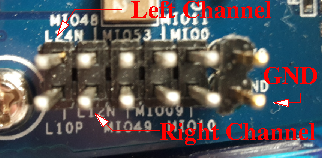
\includegraphics[width=1.\textwidth]{pluto_gpio_connector.pdf}
\end{minipage}
\end{minipage}
\end{frame}

\section{Conclusion}
\begin{frame}[fragile]\frametitle{Conclusion}
%\begin{minipage}[t]{\linewidth}
%\begin{minipage}{.65\linewidth}
{\footnotesize
\begin{itemize}
\item OscimpDigital as a {\bf flexible framework} 
for assembling signal processing
blocks on the FPGA in charge of collecting radiofrequency data
\item Platform {\bf independence} (useful investment for Intel/Altera SoC as well)
\item {\bf Consistent} IP--Linux kernel module--library--userspace application
%\item Application to GPS decoding (dual channel, acquisition step) as SatCom
%demonstration
\item {\bf Perspective}:
\begin{itemize}
\item finalize/validate GNSS parallel Gold Code correlation to ADRV9361 (Zynq 7035 $\gg$ 7010)
\item improve documentation
\item demonstration with FPGA standalone and RiscV softcore
\end{itemize}
\end{itemize}
}
%\vfill
%\fbox{\parbox{\linewidth}{
%Users {\bf not familiar with VHDL will benefit} from this framework since functional
%processing blocks are provided
%}}
%\end{minipage}
%\begin{minipage}{.34\linewidth}
%~~~\includegraphics[width=\linewidth]{A4logos.png}
%
%~~~~~~{\bf\footnotesize EU GNU Radio Days}
%\end{minipage}
%\end{minipage}
%
\vspace{0.1cm}
\noindent{\bf Resources:}

{\footnotesize
{\url{https://github.com/trabucayre/redpitaya}} (Buildroot BR2\_external)

{\url{https://github.com/oscimp/PlutoSDR}} (Buildroot BR2\_external)

{\url{https://github.com/oscimp/oscimpDigital}} (IP, driver, lib, tools \& doc)
}

\vfill
\noindent{Clone repository and submodules:}

{\footnotesize
{\verb!git clone --recursive https://github.com/oscimp/oscimpDigital.git!}
}
%\vskip
\begin{center}
{\bf Acknowledgement: PIA platform grant OscIMP}
\end{center}
\end{frame}

\end{document}
